%!TEX program = xelatex
% This is a small sample LaTeX input file (Version of 10 April 1994)
%
% Use this file as a model for making your own LaTeX input file.
% Everything to the right of a  %  is a remark to you and is ignored by LaTeX.
 
% The Local Guide tells how to run LaTeX.
 
% WARNING!  Do not type any of the following 10 characters except as directed:
%                &   $   #   %   _   {   }   ^   ~   \   
 
%\documentclass{article}        % Your input file must contain these two lines 
\documentclass[12pt, a4paper, oneside]{ctexart}
\usepackage{xeCJK}

\usepackage{indentfirst, abstract, appendix} %首行缩进
\usepackage{graphicx} %插入图片
\usepackage{amsmath, amssymb, geometry} 
\usepackage{listings, xcolor} %代码高亮
\graphicspath{{../graphics/}}
\linespread{1.2}
\geometry{left=2.5cm, right=2.5cm, top=2.5cm, bottom=2.5cm}
\title{\textbf{SVM的数学推导和Python实现}}
\author{赵新锋}
\date{\today}
\renewcommand{\abstractname}{\Large\textbf{摘要}}
\pagestyle{plain}

\lstset{ %
language=Python,                % the language of the code
basicstyle=\footnotesize,           % the size of the fonts that are used for the code
%numbers=left,                   % where to put the line-numbers
%numberstyle=\tiny\color{gray},  % the style that is used for the line-numbers
stepnumber=2,                   % the step between two line-numbers. If it's 1, each line 
                                % will be numbered
numbersep=5pt,                  % how far the line-numbers are from the code
backgroundcolor=\color{white},      % choose the background color. You must add \usepackage{color}
showspaces=false,               % show spaces adding particular underscores
showstringspaces=false,         % underline spaces within strings
showtabs=false,                 % show tabs within strings adding particular underscores
frame=single,                   % adds a frame around the code
rulecolor=\color{black},        % if not set, the frame-color may be changed on line-breaks within not-black text (e.g. commens (green here))
tabsize=2,                      % sets default tabsize to 2 spaces
captionpos=b,                   % sets the caption-position to bottom
breaklines=true,                % sets automatic line breaking
breakatwhitespace=false,        % sets if automatic breaks should only happen at whitespace
title=\lstname,                 % show the filename of files included with \lstinputlisting;
                                % also try caption instead of title
keywordstyle=\color{blue},          % keyword style
commentstyle=\it\color[RGB]{0,96,96},                % 设置代码注释的格式
stringstyle=\rmfamily\slshape\color[RGB]{128,0,0},         % string literal style
escapeinside={\%*}{*)},            % if you want to add LaTeX within your code
morekeywords={*,...}               % if you want to add more keywords to the set
}
\begin{document}               % plus the \end{document} command at the end.
\maketitle

\setcounter{page}{0}
\maketitle
\thispagestyle{empty}

\begin{abstract}
支持向量机(support vector machines, SVM)是一种分类模型,该模型在特征空间中求解间隔最大的分类超平面。
\par\textbf{关键词:}支持向量机; SVM; SMO; 矩阵运算; 矩阵求导;numpy;sklearn. 
\end{abstract}

\newpage
\pagenumbering{Roman}
\setcounter{page}{1}
\tableofcontents
\newpage
\setcounter{page}{1}
\pagenumbering{arabic}


\newpage
\section{数学推导与python实现}

\subsection{线性可分}
三层网络简单说明如下:
\begin{itemize}
    \item 输入层,不做处理,只是输入数据
    \item 隐藏层,单元数为 $ n_h $ 我们就以RELU为激活函数,另外一个常用的是sigmoid,我们把激活函数封装成一个类,可以随时替换 
    \item 输出层为一个单元,由于是二分类,我们就用sigmoid拟合对应类1的概率
\end{itemize}
\begin{figure}[htbp]
    \centering
    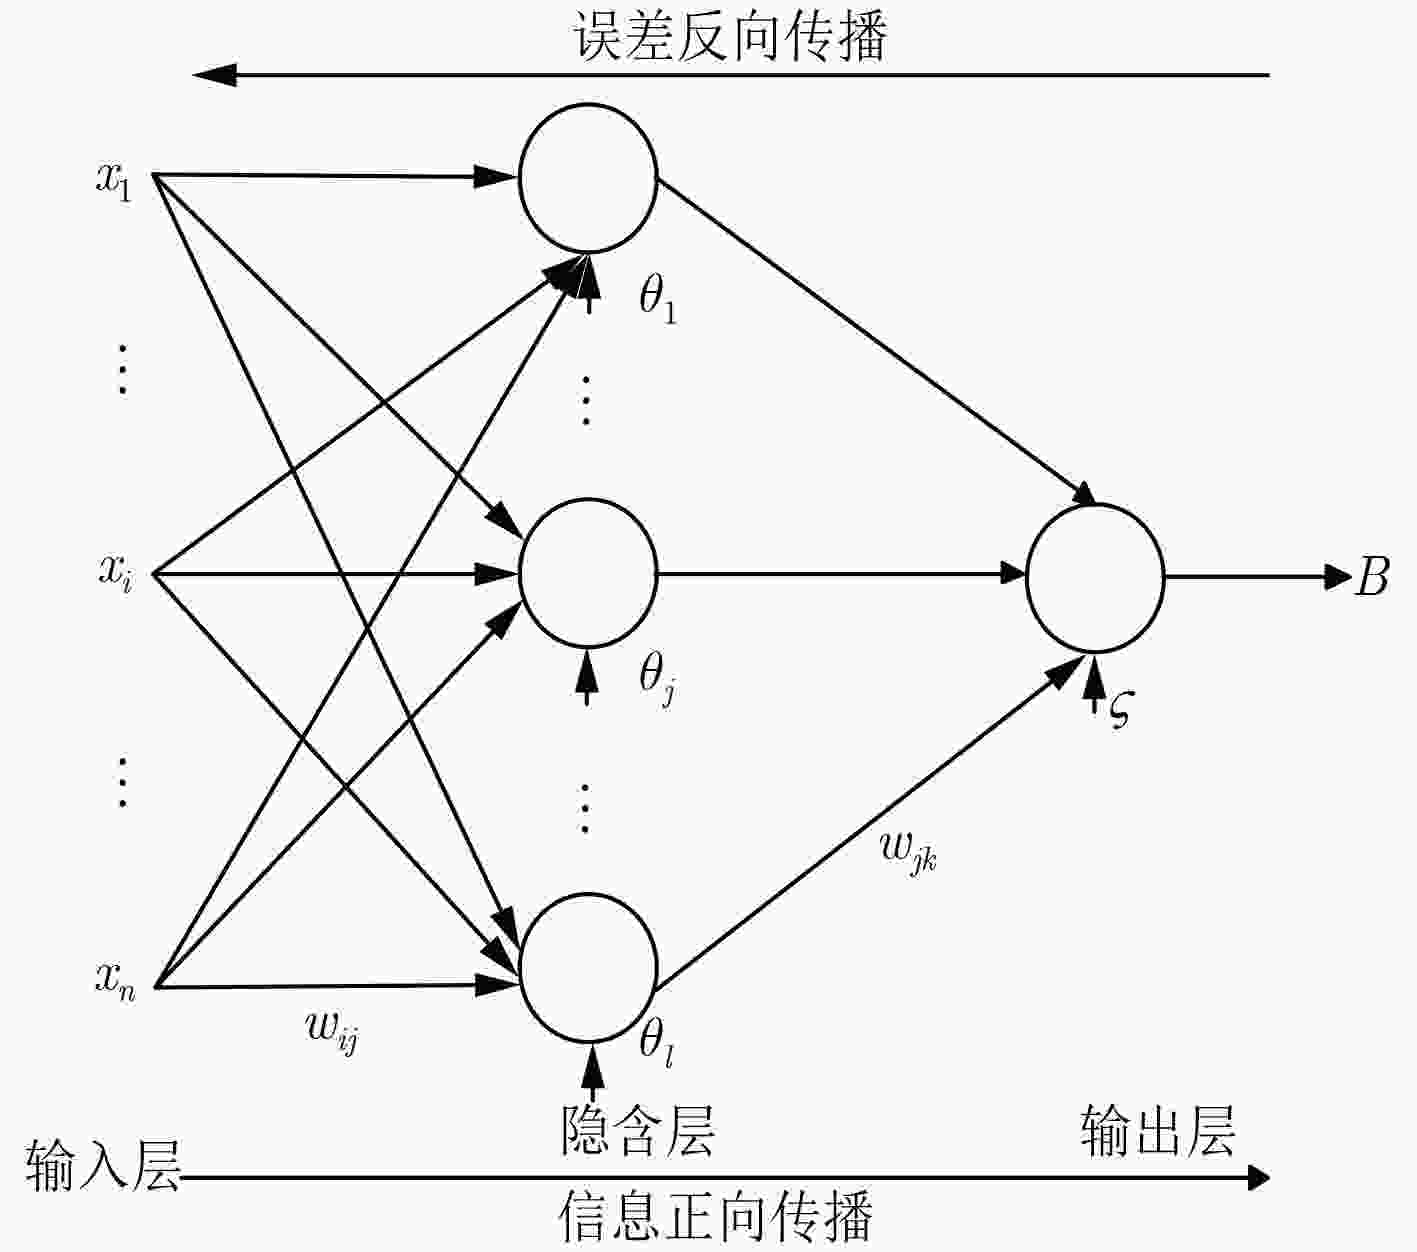
\includegraphics[width=14cm]{bpnn.png}
    \caption{神经网络示意图}\label{fig1}
\end{figure}


\begin{itemize}
\item $X$ 表示输入样本向量矩阵,$Y$表示样本集的期望输出标记(有可能是0/1标记的向量,有可能是onehot的矩阵),本文示例由于是二分类,那么Y的每个元素要么是0要么是1,$Y$是m个元素的向量,但是在运算中为了通用将其转换为$m\times 1$的矩阵。
\item $m$为样本数量,$n$为样本向量的维度。
\item 激活函数用$f$表示,隐藏层激活函数$f_h$使用RELU函数:$f_h(x) = max(0, x)$,输出层$f_o$为sigmoid函数,输出为1类的概率$f_o(x) = \frac{1}{1+exp(-x)}$
\item 隐藏层输出为$Y_h$,输出层的输出为$Y_o$
\item 隐藏层单元的参数为$w_h$, $N_h$个隐藏层单元的参数矩阵为$W_h$,输出层单元的参数为$w_o$,$N_o$个输出层单元的参数矩阵为$W_o$。
\item 虽然本文使用二分类即输出单元为1个,但是仍然使用矩阵$Yo $ 和 $ W_o$表示,从而使得算法是通用的,改成onehot+softmax方式的多分类,也是适用的。
\item 从输入到输出的公式:$Y_o = f_o(f_h(X \cdot W_h) \cdot Wo)$
\item 注:这里的线性变换$X \cdot W_h$并没有使用偏置,通过在$X$增加一个全1的列,达到同样的效果。
\end{itemize}


\subsection{公式推导}
单个样本的运算过程表示如下:    
\begin{align}
    \mathop{\arg\max}_{w_0} \ d &= \frac{y_0 \cdot (x_0^T \cdot w_0 + b_0)}{ \left\|w_0\right\|} 			\nonumber\\
	\mathrm{ s.t. }\ \   &\frac{y_i \cdot (x_i^T \cdot w_0 + b_0)}{ \left\|w_0\right\|} \geq d				\nonumber\\
	w &= \frac{w_0 }{ y_0 \cdot (x_0^T \cdot w_0 + b_0)} 			\nonumber\\
    b &= \frac{b_0 }{ y_0 \cdot (x_0^T \cdot w_0 + b_0)} 			\nonumber\\
	\mathop{\arg\max}_{w} \ d &= \frac{1}{ \left\|w\right\|} 	\iff \mathop{\arg\min}_{w} \ \left\|w\right\|		\nonumber\\
    \mathrm{ s.t. }\ \   & y_i \cdot (x_i^T \cdot w + b) \geq 1				\nonumber\\
    \mathop{\arg\min}_{w,b} \ 	L(w, b, {\alpha}) &= \frac{1}{2}	w^T \cdot w  - {\alpha} ^T \cdot  (y \odot (X \cdot w + b) - 1) \nonumber\\
        &= \frac{1}{2}	w^T \cdot w  - (\alpha \odot y) ^T \cdot  (X \cdot w + b) - \alpha^T \cdot \boldsymbol{1}^m \nonumber\\
        &= \frac{1}{2}	w^T \cdot w  - (\alpha \odot y) ^T \cdot  (X \cdot w + b) - \boldsymbol{1}^T\cdot\alpha \nonumber\\
    \mathrm{d}L &= \frac{1}{2}((\mathrm{d}w)^T \cdot w + w^T \cdot \mathrm{d}w) - (\alpha \odot y) ^T \cdot(X\mathrm{d}w) \nonumber \\
                & \ \ \  - (\alpha \odot y) ^T \cdot \mathrm{d}b \nonumber\\
                & \ \ \  - (\mathrm{d}\alpha)^T \cdot (y \odot (X \cdot w + b) - 1) \nonumber \\
                &= w^T\mathrm{d}w - (X^T\cdot(\alpha \odot y))^T\mathrm{d}w - (\alpha \odot y) ^T \cdot \mathrm{d}b - (y \odot (X \cdot w + b) - 1)^T\mathrm{d}\alpha \nonumber \\
    \frac{\partial L}{\partial w} &= w - X^T\cdot(\alpha \odot y) \nonumber \\
    \frac{\partial L}{\partial b} &= - \alpha \odot y \nonumber \\
    \iff \nonumber \\
    w &= X^T\cdot(\alpha \odot y) \nonumber \\
    \alpha \odot y &= \boldsymbol{0} \nonumber \\
    \mathop{\arg\max}_{\alpha} L(w, b, {\alpha}) &= \frac{1}{2}(\alpha \odot y)^T \cdot X^T \cdot X \cdot (\alpha \odot y) \nonumber \\
                      & \ \ \  - (\alpha \odot y)^T \cdot X^T \cdot X \cdot (\alpha \odot y) \nonumber \\
                      & \ \ \  - (\alpha \odot y)^T \cdot b^m  \nonumber \\
                      &= -\frac{1}{2}(\alpha \odot y)^T \cdot X^T \cdot X \cdot (\alpha \odot y) + (\alpha \odot y^T) \cdot b \nonumber \\
                      &= -\frac{1}{2}(\alpha \odot y)^T \cdot X^T \cdot X \cdot (\alpha \odot y) \nonumber \\
    \iff \mathop{\arg\min}_{\alpha} L(w, b, {\alpha}) &= \frac{1}{2}(\alpha \odot y)^T \cdot X^T \cdot X \cdot (\alpha \odot y) \nonumber \\
        \mathrm{ s.t. }\ \   \alpha \odot y &= \boldsymbol{0} \nonumber \\
\end{align}
\begin{align}
    L(w, b, {\alpha}, u) &= \frac{1}{2}w^T \cdot w + C \cdot \xi^T \cdot\boldsymbol{1}^m   - {\alpha} ^T \cdot  (y \odot (X \cdot w + b) - 1) - u^T \cdot \xi \nonumber \\
    \frac{\partial L}{\partial w} &= w - X^T\cdot(\alpha \odot y) \nonumber \\
    \frac{\partial L}{\partial b} &= - \alpha \odot y \nonumber  \\
    \frac{\partial L}{\partial \xi} &= C - \alpha - u \nonumber \\
    \iff  L(w, b, \xi, {\alpha}, u) &= -\frac{1}{2}(\alpha \odot y)^T \cdot X^T \cdot X \cdot (\alpha \odot y) + \boldsymbol{1}^m \cdot \alpha \nonumber \\
    \mathrm{ s.t. }\ \   \alpha \odot y &= \boldsymbol{0} \nonumber \\
    C - \alpha - u \nonumber  = \boldsymbol{0} \nonumber \\
    \alpha_i \geq 0 \nonumber \\
    u_i \geq 0 \nonumber 
\end{align}

End!!




\end{document}                 % The input file ends with this command.

